%!TEX root = thesis.tex
\chapter{Conclusions}
\label{chap:conc}
\section{Impact of Dissertation}
The work presented in this dissertation comprises of models of thermal conduction in a number of semiconductor nanostructures, beginning with incorporating surface descriptors to create predictive models and bridge the differences between experimental and computational research, to uncovering a novel phonon coupling mechanism to modulate thermal transport in layered nanomaterials. While we primarily utilized silicon and germanium as elements of choice, the general insights about the flow of heat in different nanostructures are applicable across a wide range of semiconductors. 

\par The lack of existing predictive models that could account for all the relevant physical descriptors in the phonon-surface scattering motivated the study in \Cref{chap:predictive}. The objective of creating phonon transport models which rely on experimentally quantifiable surface descriptors (i.e. surface roughness and correlation length) and embody key physics of phonon-transport (i.e. surface scattering dependence on incident phonon momentum, incident angle and do not treat internal and surface scattering as volumetric phenomena) was achieved with the use of Beckmann-Kirchhoff surface scattering theory along with surface shadowing correction. After developing the phonon-surface scattering model, we showed that the model accurately agrees with the experimentally thermal conductivities of nanowires and thin-films. Moving beyond the traditionally measured thermal conductivity, we predicted that a decrease in the nanostructure size and increased roughness and correlation lengths makes the thermal spectra significantly shift towards phonons with short wavelengths and mean-free-paths. The versatility of the predictive model was highlighted by the results of thermal spectra for bulk materials, which showed excellent agreement with recent experimental approaches that reconstruct the mean-free-path heat spectra. Our predictions showed how the specific surface properties and temperatures can significantly modify the thermal conductivity accumulation, thereby opening a way forward to the rational design of the semiconductor-air interfaces, which can be utilized to tailor the desired thermal transport properties in nanostructures. 

\par We extended the phonon-transport model in \Cref{chap:diff_boundary} to move beyond the assumption of symmetric boundaries in thin-films, with the motivation of a better replication of typical experimental nanostructures. The methods developed move beyond the commonly used diffuse scattering surface assumptions, enabling the surfaces of the thin films to be precisely described via their individual specularities. Furthermore, during this development, we highlighted the equivalence of solving the Boltzmann transport equation by explicitly calculating mean-free-paths or by utilizing the boundary conditions to semi-analytically evaluate non-equilibrium phononic populations. The latter approach is utilized in layered materials discussed in \Cref{chap:layered,chap:slxp}. Our primary objective was to analyze the spatial distribution of thermal flux in asymmetric thin-films.We showed that designing the physical properties of thin-film surfaces provides control over the preferential spatial location of thermal flux, which could hold significant potential for rational design of thermal materials. Additionally, we showed the existence of heat transport regimes, controlled by the surface properties resembling fluid flow in confined geometries.
 
\par Our ability to model asymmetric structures proved central in quantitatively predicting thermal transport in nanotubes in \Cref{chap:nt}. Semiconductor nanotubes present an exciting avenue to create very thin one-dimensional nanostructures using currently available growth techniques. Due to their large surface-to-volume ratio, nanotubes allow for an effective control over thermal energy transfer. The ability to treat the two boundaries of the nanotubes as distinct from one another allowed us to discriminate between phonon modes that depended on the properties of both the boundaries (NT-modes) and those that were independent of the inner boundary (NW-modes). The versatility of our model allowed us to analyze the impact of nanotube morphology such as shell thicknesses, outer diameters, and surface properties on thermal transport. We concluded that in general, the thermal conductivity of the nanotube depends on the outer diameter even for the same shell thickness. We showed that the experimentally observed independence between these quantities could be explained by a combination of addition of impurity atoms to the Silicon lattice and surface roughness. We also evaluated the frequency and mean-free-path spectra to elucidate and provide insight on the phonon transport mechanisms in low-dimensional nanotube structures.

\par The phonon-surface scattering in all of the nanostructures discussed serves to reduce thermal transport by shortening phononic mean-free-paths. Motivated by the central question, is it possible to increase phononic-mean-free-paths at the nanoscale, we explored thermal transport in layered nanomaterials in \Cref{chap:layered}. We showed that enhanced thermal conductivities can be achieved in semiconductor nanostructures by rationally engineering phonon spectral coupling between materials. By embedding a germanium film between silicon layers, we showed that its thermal conductivity could potentially be increased by more than 100\% at room temperature in contrast to a free standing thin-film and the injection of phonons from the cladding silicon layers created the observed enhancement in thermal conductivity. While analyzing the underlying phonon-injection mechanism we found that the aforesaid increase comes at the cost of a reduction of thermal conductivity of the silicon layers. Our evaluations of the dependence of thermal conductivity modulations of both silicon and germanium layers on structural parameters showed the critically role of layer spacings and interface properties. Thus, we showed a novel phonon-surface behavior beyond the traditional diffusive scattering of phonons that can be tuned to modulate thermal transport. Next, we extended the tri-layer transport analysis to bi-layer structures to elucidate thermal transport in structures of technological importance, i.e. film-on-substrate (FOS) architectures. We observed an unconventional behavior of thermal conductivity variation with film thickness, an increased thermal conductivity with decreasing thickness in \algas{0.1}{0.9} films over GaAs substrate. In contrast, Ge films over Si substrate showed a decreasing thermal conductivity with decreasing thickness. The difference in behavior arose due to the phonon injection from substrate media which is critically dependent on the interplay of acoustic impedance mismatch, materials thermal transport properties, interfacial characteristics, and thickness of thin film atop the substrate. We also determined that a trade-off between interfacial scattering and available volume fraction for enhancement play a crucial role in determining the thermal conductivity of the FOS. The analysis of the FOS architectures suggests that experimental measurement of thermal conductivity of thin-films needs to account for thermal coupling between thin film and substrate and the consequent conductivity modification and highlights the need to develop rigorous conductivity read-out models for experiments.

\par Lastly, we utilized our models of layered nanomaterials to study cross-plane thermal conduction in silicon-germanium superlattices considering interactions of phonons with multiple structural length scales in \Cref{chap:slxp}. Our results clearly highlighted the need for quantifying the impact of all relevant length variables in superlattices, i.e., the mean-free-path and wavelength of phonons, the periodicity of the structure, total size of the superlattice, and the length scale of interfacial disorder, to fully understand the heat conduction in superlattices. Our predictions showed that thermal conduction can be ballistic traveling across multiple low roughness interfaces of the superlattice even at room temperatures. In contrast to in-plane transport, we found that the strong surface scattering encountered in the cross-plane direction limits the phonon transport to mean-free-paths of less than 1 \si{\micro}m and wavelengths less than 10 nm even in alloyed superlattices of periods up to 50 nm. This strong role of boundaries also manifests itself in the form of thermal conductivity anisotropy in superlattices. We also reported the impact of the number of periods and total structural size on the thermal conductivity which is critical for accurate experimental reporting of thermal conductivities.

\section{Possible Directions for Future Work}
There are several interesting research projects that are natural extensions of the work presented in this thesis:

\subsection{Exploring the Limits of Phonon Injection Mechanism}
The complex nature of phonon injection mechanism manifests itself in unique and novel changes to thermal conductivities as highlighted in this thesis. Both the structural properties which include layer thicknesses and surfaces roughness, and the the material properties which involve the dispersion relations and relaxation times, are important to this mechanism.  Further study can help elucidate this mechanism to understand the limits of phonon coupling. For instance, transmission of phonons across interfaces requires propagating modes in both materials. From this perspective, materials with similar phononic dispersions would create a greater degree of phonon spectral coupling. Additionally, we showed that small surface roughness and consequential lower diffusive scattering of phonons increase the spectral coupling between the two materials. Thus, materials with similar lattice constants would favor effective phonon spectral coupling by providing smoother interfaces. Also, the difference in thermal transport properties gives rise to the concept of net phonon injector and acceptor roles for materials. Hence, the search for a system to observe maximized thermal conductivity enhancement and reduction effects would need to account for both the degree of phonon coupling and the difference in thermal properties. For instance, coupling a given material with an extremely high thermal conductivity material such as diamond or graphene could exhibit unique thermal conductivity modulations.  

\subsection{Guided Experiments for Validating Thermal Conductivity Enhancement Predictions}
In order to experimentally validate the predictions of thermal conductivity enhancement presented in this thesis, collaborative effort to fabricate samples with controlled surface disorder and measure layer-by-layer thermal conductivity would be required. In this regard, thermal conductivity measurements on thin-film grown on substrates may provide a better platform since they are better studied and thermoreflectance measurement techniques can be used to validate the findings. Considerations on the ability to fabricate specified layer thicknesses while preserving control over surface properties would need to be kept in mind and typical read-out models from experiments that ignore phonon coupling may need to be improved in order to quantitatively validate the predictions. Concurrently, a sequence of samples with different layer spacings may be utilized to qualitatively validate the predictions presented in this thesis.

\subsection{Coherent Phonons and their Impact on Thermal Transport}
The modulations of thermal transport in this thesis have stemmed from changes in transport properties of phonons that are uncorrelated with their phase, i.e. by considering the particle like behavior of phonons in the form of their mean-free-paths. However, under certain conditions, it is possible for phonons to exhibit coherent interference phenomenon which can manipulate their heat carrying ability by changing the phonon dispersion relations, thereby altering the phonon group velocities and density of states \cite{RN132,RN362}. We estimated the potential impact of such coherent behavior in the form of quantum confinement in thin-films by extracting information from thermal spectra in this thesis. However, in order to provide rigorous calculations further research is needed to account for these changes within a thermal transport model. In particular, the cross-plane transport in superlattices has been shown to be influenced by coherent interference of phonons \cite{RN393}. The presence of smooth surfaces that avoids diffuse scattering favors such coherent interference of phonons \cite{RN132,RN362} allowing the phonons to traverse multiple interfaces. Furthermore, thermal spectra can be tuned so that phonons with lower frequencies and longer mean-free-paths dominate thermal transport, allowing for coherent effects to be strongly expressed. Coherent modifications to phonon transport coupled with the transport models developed in this thesis would encompass the possible scope of modulating thermal transport via nanostructuring in semiconductors.
\todo{Discuss with MM, if need more, possibly combining conduction, convection and radiation effects?}
\par These are just a few of the possibilities that could present exciting avenues for research. As the understanding of phonon transport and the ability to engineer novel nanostructures continues to evolve, it is our hope that this thesis will provide a firm foundation for future exploration of engineering the flow of heat at the nanoscale.

%%Eqn.
%\begin{equation}
%  \sum_{i=1}^{n}{(X_i - \overline{X})^2}^{n}{(X_i - \overline{X})^2}\ . 
%\end{equation}
%
%
% This is a figure
%\begin{figure}
%	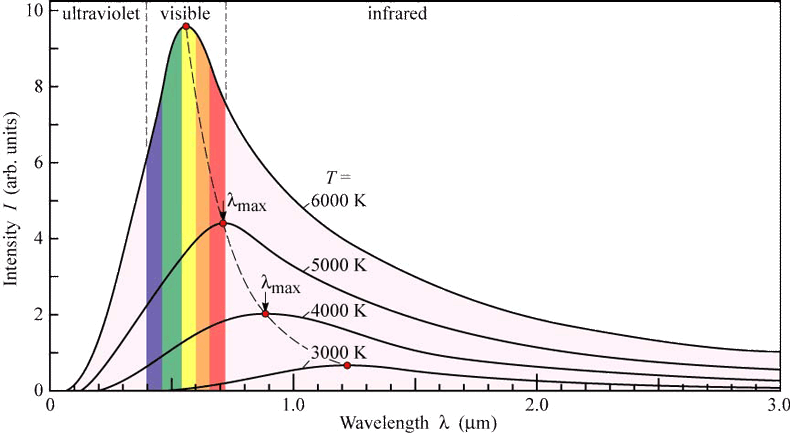
\includegraphics[width=\textwidth]{exampleFigure.png}
%	\caption{This is an example Figure.}
%	\label{Figure in Chapter 6}
%\end{figure}
%
%\begin{equation}\label{key}
%\sqrt{\cos(x)}=1
%\end{equation}
%This implies that,
%\begin{equation}\label{eq:test}
%\boxed{\text{Free particle is: } K_{k+1}=P_ka_{k+1}^T\left(a_{k+1}P_ka_{k+1}^T+I_N\right)^{-1}}
%\end{equation}
%
%\begin{equation}\label{eq:test2}
%\boxed{\text{Free particle is: }\  \Psi(\mathbf{x},t)=e^{i(\mathbf{k}.\mathbf{x}-\omega t)}}
%\end{equation}
%
%\begin{equation} \label{tranfdc}
%\begin{split}
%T_v(s) & = \frac{V_{dc}(s)}{V_{dcref}(s)}
%= \frac{\omega _B}{B}
%\frac{k_{pdc}s + k_{idc}} {s^2 + \frac{ k_{pdc} \omega _B s} {B} +
%	\frac{k_{idc} \omega _B} {B}} ,  \\
%%
%T_i(s) & = \frac{V_{dc}(s)}{i_{l}(s)}
%= - \frac{\omega _B}{B} \frac{s} {s^2
%	+ \frac{ k_{pdc} \omega _B s} {B} + \frac{k_{idc} \omega _B} {B}} .
%\end{split}
%\end{equation}
%
%
%\begin{align*}
%x&=y           &  w &=z              &  a&=b+c\\
%2x&=-y         &  3w&=\frac{1}{2}z   &  a&=b\\
%-4 + 5x&=2+y   &  w+2&=-1+w          &  ab&=cb
%\end{align*}
